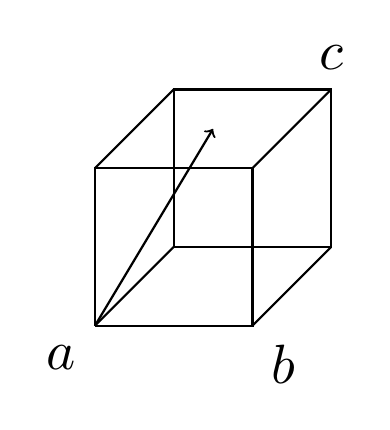
\begin{tikzpicture}
    % Define points for the cube
    \coordinate (A) at (0,0);
    \coordinate (B) at (2,0);
    \coordinate (C) at (2,2);
    \coordinate (D) at (0,2);
    \coordinate (E) at (1,1);
    \coordinate (F) at (3,1);
    \coordinate (G) at (3,3);
    \coordinate (H) at (1,3);

    % Draw edges of the cube
    \draw[thick] (A) -- (B) -- (C) -- (D) -- (A); % Bottom square
    \draw[thick] (E) -- (F) -- (G) -- (H) -- (E); % Top square
    \draw[thick] (A) -- (E); % Left edge
    \draw[thick] (B) -- (F); % Right edge
    \draw[thick] (C) -- (G); % Top right edge
    \draw[thick] (D) -- (H); % Top left edge
    \draw[->,thick](A) -- (1.5,2.5);
    % Labels
    \node[below left, scale=2] at (A) {$a$};
    \node[below right, scale=2] at (B) {$b$};
    \node[above, scale=2] at (G) {$c$};
\end{tikzpicture}
